\section{Introduction}
\label{sec:introduction}


%KVS popular and widely used
%Example KVS
%Scope KVS for this paper
%But for all their benefits, limited query language
%For example, no SQL, such as ..., often required to do X, Y. Z
%Point solutions exist, e.g., ..., drawbacks
%Approach in this paper, different from above
%Contributions
%Outline

%KVS popular and widely used
The properties of major Internet players are backed by what has
become known as \textit{key-value stores} (\KVSs), handling millions
of client requests and producing terabytes of data on a daily
basis~\cite{parikh:facebook}.
%
%Example KVS
%
Examples include Google's Bigtable\cite{chang:bigtable}, Amazon's
Dynamo~\cite{decandia:dynamo}, Yahoo's PNUTS~\cite{cooper:pnuts},
Apache's HBase~\cite{george:hbase}, and
Cassandra~\cite{hewitt:cassandra} which originated at Facebook.

%
%Scope KVS for this paper
%

As opposed to earlier generation key-value stores, such as
\textsf{BerkeleyDB}, which were more intended as main-memory databases
to persist application configurations, among others, the \KVSs\ we
consider in this paper are highly distributed and large-scale systems
designed to back today's massive-scale Internet services.

%
%But for all their benefits, limited query language
%

These \KVSs\ are highly available and provide advanced features like
load balancing and fault-tolerance~\cite{chang:bigtable,
  decandia:dynamo, cooper:pnuts, george:hbase, hewitt:cassandra}.  For
example, \KVSs\ scale horizontally by partitioning data and request
load across a configurable number of nodes. To achieve these
properties at scale, \KVSs\ sacrifice, among others, an expressive
query language and data model, only offering a simple API, comprising
\textit{get}, \textit{put}, and \textit{delete} operations.
%
%For example, no SQL, such as ..., often required to do X, Y. Z
%
While this design offers efficient access to single row entries,
the processing of more complex SQL-like queries, such as, selection,
projection, aggregation, and join, require costly application-level
operations. For example, to compute a join, the tables to be joined
have to be read by the application, joined, and written back to the
store, unless result storage is not required.

%
%Point solutions exist, e.g., ..., drawbacks
%

Point solutions have appeared that raise the level of abstraction of a
given \KVS\ by partially or fully materializing desired
application-level queries as views through the underlying
store~\cite{agrawal:asynchronous, silberstein:feeding,
  phoenix:apache}.  In this manner, secondary indices have been added
to \KVSs~\cite{agrawal:asynchronous, kejriwal:slik}, caching of
application queries has been enabled~\cite{kate:easy}, massive
processing of selection views for feed following applications has been
enabled~\cite{silberstein:feeding}, however, a generic solution that
introduces view management for a wide variety of SQL query operators
as views to \KVS\ is still at large.

\begin{figure} 
	\centering 
	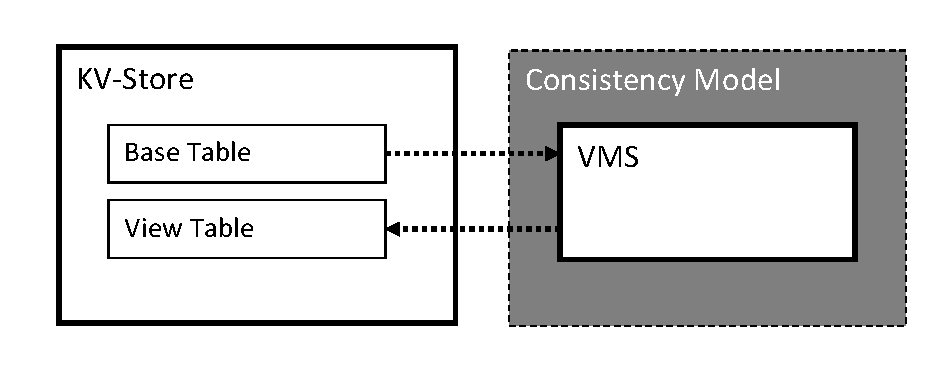
\includegraphics[width=\linewidth]{figures/ResearchGoal} 
	\vspace{-10mm} 
	\caption{System overview} 
	\vspace{-3mm} \label{fig:research_goal} 
\end{figure} 

%
%Approach in this paper, different from above
%

It is this problem that this paper addresses.  As opposed to existing
solutions, our design abstracts from a specific \KVS, aiming to
support a whole gamut of \KVSs\ that offer a small set of key features
our design leverages.

%Our approach
Our approach introduces mechanisms for the materialization and
incremental maintenance of views to \KVSs\ resulting in sophisticated
query capabilities for applications, simply through definition of view
expressions.  Materialized views are tables managed by the \KVS\ and
all properties such as concurrent access, availability, and
fault-tolerance, apply to views as well.  Views are maintained
incrementally: base data updates propagate through the system to only
effect the derived view data records.  The challenge is the design of
the \textit{View Maintenance System} (\VMS) that efficiently and
correctly maintains views at the desired scale. We developed such a
system, as shown in Figure~\ref{fig:research_goal}.  \VMS\ consumes
streams of client base data operations and produces updates to view
data records.

%
% aj - above - I exceptionally capitalized VMS above to hint at it
%              being a name.
%




%Contributions
%
% aj - claims are a bit strong, especially, the first
%       one
%      the last one could benefit from a stronger
%       insight about the results; negligible overhead is
%       a bit strong
% We'll leave it at this for now.
%
This paper makes the following contributions:
%
(1) We provide an analysis of popular \KVSs\ to identify a small set
of common features, a generic \VMS\ design requires to correctly
materialize views (cf.  Section~\ref{sec:kv_model}.)
%
(2) We design \VMS\ in the spirit of existing \KVSs\ to offer
horizontal scalability and fault-tolerance by simply leveraging the
existing mechanisms of the stores
(cf. Section~\ref{sec:view_maintenance_system}.)
%
(3) We introduce novel concepts, namely auxiliary views, as basis for
correctly and consistently materializing views in
\KVSs\ (cf. Section~\ref{sec:view_maintenance}.)
%
(4) We validate \VMS\ by extending \HB\ with view maintenance
capabilities and demonstrate that the extended architecture is at par
in terms of performance with plain \HB\ at negligible overhead
(cf. Section~\ref{sec:evaluation}.)

%Outline
%Included above due to space limitations



